\section{Теорема Пифагора}

\paragraph{}\label{1938/188}
\so{Теорема}.
\textbf{\emph{В прямоугольном треугольнике перпендикуляр, опущенный из вершины прямого угла на гипотенузу, есть средняя пропорциональная величина между отрезками, на которые основание перпендикуляра делит гипотенузу, а каждый катет есть средняя пропорциональная между гипотенузой и прилежащим к этому катету отрезком гипотенузы.}}

Пусть $AD$ (рис.~\ref{1938/ris-198}) есть перпендикуляр, опущенный из вершины прямого угла $A$ на гипотенузу $BC$.
Требуется доказать следующие три пропорции:
\begin{align*}
1)\ \frac{BD}{AD}&=\frac{AD}{DC};
&
2)\ \frac{BC}{AB}&=\frac{AB}{BD};
&
3)\ \frac{BC}{AC}&=\frac{AC}{DC}.
\end{align*}

\begin{wrapfigure}{o}{45mm}
\centering
\includegraphics{mppics/ris-198}
\caption{}\label{1938/ris-198}
\end{wrapfigure}

Первую пропорцию мы докажем из подобия $\triangle ABD\sim \triangle CAD$.
Эти треугольники подобны, потому что
\[\angle 1 = \angle 4\quad \text{и} \quad\angle 2 = \angle 3.\]
вследствие перпендикулярности их сторон (§~\ref{1938/80}).
Возьмём в $\triangle ABD$ те стороны $BD$ и $AD$, которые составляют первое отношение доказываемой пропорции;
соответственными сторонами в $\triangle CAD$ будут $AD$ и $DC$%
\footnote{Чтобы безошибочно определить, какие стороны взятых треугольников соответственны между собой, полезно держаться такого пути:

1) указать углы, против которых лежат взятые стороны одного треугольника.

2) найти равные им углы в другом треугольнике.

3) взять противолежащие им стороны.

Например, для треугольников $ABD$ и $CAD$ рассуждаем так:
в треугольнике $ABD$ стороны $BD$ и $AD$ лежат против углов 1 и 3;
в треугольнике $CAD$ этим углам равны 4 и 2;
против них лежат стороны $AD$ и $DC$.
Значит, стороны $AD$ и $DC$ соответственны сторонам $BD$ и $AD$.
}%
, поэтому
\[\frac{BD}{AD}=\frac{AD}{DC}.\]

Вторую пропорцию докажем из подобия $\triangle ABC\sim \triangle DBA$.
Эти треугольники подобны, потому что они прямоугольные и острый угол $B$ у них общий.
В $\triangle ABC$ возьмём те стороны $BC$ и $AB$, которые составляют первое отношение доказываемой пропорции;
соответственными сторонами в $\triangle DBA$ будут $AB$ и $BD$;
поэтому
\[\frac{BC}{AB}=\frac{AB}{BD}.\]

Третью пропорцию докажем из подобия $\triangle ABC\sim \triangle DAC$.
Эти треугольники подобны, потому что они оба прямоугольные и имеют общий острый угол $C$.
В $\triangle ABC$ возьмём стороны $BC$ и $AC$;
соответственными сторонами в $\triangle DAC$ будут $AC$ и $DC$;
поэтому
\[\frac{BC}{AC}=\frac{AC}{DC}.\]

\paragraph{}\label{1938/189}
\mbox{\so{Следствие}.}
Пусть $A$ (рис.~\ref{1938/ris-199}) есть произвольная точка окружности, описанной на диаметре $BC$.
Соединив концы диаметра с этой точкой, мы получим прямоугольный треугольник $ABC$, у которого гипотенуза есть диаметр, а катеты образованы хордами (§~\ref{1938/125}, \ref{1938/2}).
Применяя доказанную выше теорему к этому треугольнику, приходим к следующему заключению:

\begin{wrapfigure}{o}{36mm}
\centering
\includegraphics{mppics/ris-199}
\caption{}\label{1938/ris-199}
\end{wrapfigure}

\emph{Перпендикуляр, опущенный из какой-либо точки окружности на диаметр, есть средняя пропорциональная величина между отрезками, на которые основание перпендикуляра делит диаметр, а хорда, соединяющая эту точку с концом диаметра, есть средняя пропорциональная между диаметром и прилежащим к хорде отрезком диаметра.}

\paragraph{}\label{1938/190}
\so{Задача}.
\emph{Построить отрезок, средний пропорциональный между двумя отрезками $a$ и $b$,}
то есть построить отрезок $x$, такой, что $a:x= x:b$.

{

\begin{wrapfigure}{r}{35mm}
\vskip-4mm
\centering
\includegraphics{mppics/ris-200}
\caption{}\label{1938/ris-200}
\bigskip
\includegraphics{mppics/ris-201}
\caption{}\label{1938/ris-201}
\end{wrapfigure}

Приведём два решения.


1) на произвольной прямой (рис.~\ref{1938/ris-200}) откладываем отрезки $AB=a$ и $BC\z=b$;
на $AC$, как на диаметре, описываем полуокружность;
из $B$ восстанавливаем перпендикуляр $BD$ до пересечения с окружностью.
Этот перпендикуляр и есть искомая средняя пропорциональная между $AB$ и $BC$.

2) на произвольной прямой (рис.~\ref{1938/ris-201}) откладываем от точки $A$ отрезки $a$ и $b$.
На большем из этих отрезков описываем полуокружность.
Проведя из конца меньшего отрезка перпендикуляр к $AB$ до пересечения его с окружностью в точке $D$, соединяем $A$ с $D$.
Хорда $AD$ есть средняя пропорциональная между $a$ и $b$.

}

\paragraph{Теорема Пифагора.}\label{1938/191}
Доказанные выше теоремы позволяют обнаружить замечательное соотношение между сторонами любого прямоугольного треугольника.
Это соотношение названо в честь греческого геометра Пифагора (VI век до нашей эры).

\textbf{\emph{Квадрат длины гипотенузы равен сумме квадратов длин катетов.}} 

Пусть $ABC$ (рис.~\ref{1938/ris-202}) есть прямоугольный треугольник, $AD$ — перпендикуляр, опущенный на гипотенузу из вершины прямого угла.
Положим, что стороны и отрезки гипотенузы измерены одной и той же единицей, причём получились числа $a$, $b$, $c$, $c'$ и $b'$ (принято длины сторон треугольника обозначать малыми буквами, соответствующими большим буквам, которыми обозначены противолежащие углы).

\begin{wrapfigure}{o}{47mm}
\centering
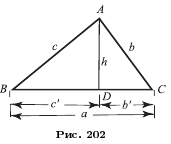
\includegraphics{mppics/ris-202}
\caption{}\label{1938/ris-202}
\end{wrapfigure}

Применяя теорему §~\ref{1938/188}, можем написать пропорции:
\[\frac ac=\frac c{c'}
\quad\text{и}\quad
\frac ab=\frac b{b'}\]
откуда 
\[a\cdot c'=c^2
\quad\text{и}\quad
a\cdot b'=b^2.\]
Сложив почленно эти два равенства, найдём:
\[a\cdot c'+a\cdot b'=c^2+b^2
\quad\text{или}\quad
a\cdot (c'+b')=c^2+b^2.\]
Но $c'+b'=a$, следовательно,
\[a^2=c^2+b^2.\]

\smallskip
\so{Пример}.
Если катеты, измеренные какой-нибудь линейной единицей, равны 3 и 4; 
тогда гипотенуза  $x$, удовлетворяет уравнению:
\[x^2=3^2+4^2=9+16=25,\]
откуда $x = \sqrt{25} = 5$.

\smallskip
\so{Замечание}.
Прямоугольный треугольник со сторонами 3, 4 и 5 называется \so{египетским треугольником}. 
Им можно пользоваться для построения прямого угла на земной поверхности:
бечёвку посредством узлов разделяем на 12 равных частей;
затем, связав концы, натягиваем её на земле (посредством кольев) в виде треугольника со сторонами в 3, 4 и 5 делений;
тогда угол между сторонами, равными 3 и 4, оказывался прямым.%
\footnote{Прямоугольные треугольники, у которых стороны измеряются целыми числами, носят название \so{пифагоровых треугольников}.
Прямые вычисления показывают, что если $a$ и $b$ — произвольные целые числа такие, что $a>b$ то для
\[x=2ab,
\quad
y=a^2-b^2,
\quad
z=a^2+b^2\]
выполнено тождество $x^2+y^2=z^2$.
В частности треугольник со сторонами $x$, $y$ и $z$ является пифагоровым.
Можно доказать, также что любой пифагоров треугольник имеет стороны $k{\cdot}x$, $k{\cdot}y$ и $k{\cdot}z$ для некоторых целых $a$, $b$ и $k$. % изменил формулировку
}

Теорема Пифагора имеет ещё другую формулировку, именно ту, которая была для неё получена самим Пифагором.
С этой формулировкой мы познакомимся позднее (§~\ref{1938/257}).

\paragraph{}\label{1938/192}
\so{Следствие}.
\emph{Квадраты катетов относятся между собой как прилежащие отрезки гипотенузы.}
Действительно, из уравнений предыдущего параграфа находим:
\[\frac{c^2}{b^2}=\frac{a\cdot c'}{a\cdot b'}=\frac{c'}{b'}.\]

\paragraph{}\label{1938/193}
\so{Замечание 1}.
К трём равенствам, которые мы вывели выше:
\[1)\ a\cdot c'=c^2;
\qquad
2)\ a\cdot b'=b^2
\quad
\text{и}
\quad
3)\ a^2=b^2+c^2,
\]
можно присоединить ещё следующие два:
\[4)\ b'+c'=a
\quad
\text{и}
\quad
5)\ h^2=b'\cdot c',
\]
(если буквой $h$ обозначим длину высоты $AD$).
Из этих равенств третье, как мы видели, составляет следствие первых двух и четвёртого, так что из пяти равенств только четыре независимы;
вследствие этого можно по данным двум из шести чисел находить остальные четыре.

Для примера положим, что нам даны отрезки гипотенузы $b' = 5 \text{м}$ и $c' = 7\text{м}$;
тогда
\begin{align*}
a&=b'+c'=12;
\\
c&=\sqrt{a\cdot c'}=
\sqrt{12\cdot 7}=
\sqrt{84}=9{,}165\dots;
\\
b&=\sqrt{a\cdot b'}=\sqrt{12\cdot 5}=\sqrt{60}=7{,}745\dots;
\\
h&=\sqrt{c'\cdot b'}=\sqrt{5\cdot 7}=\sqrt{35} = 5{,}916\dots
\end{align*}
